\documentclass[12pt,a4paper]{article}

\usepackage[utf8]{inputenc}
\usepackage[T1]{fontenc}
\usepackage{geometry}
\geometry{margin=2.5cm}
\usepackage{hyperref}
\hypersetup{
    colorlinks=true,
    linkcolor=blue,
    filecolor=magenta,
    urlcolor=cyan,
    citecolor=blue,
}
\usepackage{enumitem}
\usepackage{booktabs}
\usepackage{xcolor}
\usepackage{titlesec}
\usepackage{caption}
\usepackage{fancyhdr}
\usepackage{float}
\usepackage{tabularx}
\usepackage{tikz}
\usetikzlibrary{positioning, arrows.meta, shapes.geometric, fit, backgrounds}
\usepackage{listings}
\usepackage{amsmath}

\pagestyle{fancy}
\fancyhf{}
\lhead{Rapport Final \textemdash{} TeacherLM}
\rhead{Master SIE \textemdash{} 2026}
\cfoot{\thepage}

\titleformat{\section}{\large\bfseries\color{blue!70!black}}{}{0em}{}[\titlerule]
\titleformat{\subsection}{\bfseries\color{blue!50!black}}{}{0em}{}
\titleformat{\subsubsection}{\bfseries\color{blue!35!black}}{}{0em}{}

\lstset{
    basicstyle=\small\ttfamily,
    backgroundcolor=\color{gray!10},
    frame=single,
    breaklines=true,
    keywordstyle=\color{blue}\bfseries,
    commentstyle=\color{gray},
    stringstyle=\color{orange},
}

\title{
    \vspace{-2cm}
    \large Master Systèmes Intelligents pour l'Éducation (SIE)\\
    \vspace{0.5cm}
    \huge \textbf{Rapport d'etat d'avancement}\\
    \vspace{0.3cm}
    \LARGE \textbf{TeacherLM}\\
    \vspace{0.2cm}
    \large \textit{Plateforme de Tutorat IA Basée sur RAG Multi-Agent}
}
\author{\textbf{Étudiant :} Amine EL HANINE \\ \textbf{Encadrant :} Pr. Abdelaaziz Hessane}
\date{Avril 2026}

\begin{document}

\maketitle
\thispagestyle{empty}

\begin{abstract}
\textbf{TeacherLM} est une plateforme de tutorat intelligent full-stack qui transforme les documents de cours uploadés en un tuteur IA personnalisé. Le système s'appuie sur une architecture microservices multi-agents combinant Retrieval-Augmented Generation (RAG) hybride, inférence LLM locale via Ollama, et suivi pédagogique adaptatif. Chaque réponse est strictement ancrée dans les matériaux de cours fournis, garantissant zéro hallucination et confidentialité totale des données. La plateforme génère des contenus pédagogiques variés (quiz, cartes mentales, podcasts, flashcards) et maintient un profil d'apprenant évolutif pour adapter dynamiquement les stratégies d'enseignement.
\end{abstract}

\newpage
\tableofcontents
\newpage

\section{Vue d'ensemble du projet}

\subsection{Objectif et positionnement}

TeacherLM est un système de tutorat IA qui résout un problème fondamental dans l'éducation assistée par intelligence artificielle : comment créer un tuteur qui ne réponde \textbf{qu'à partir des documents fournis} sans inventer d'informations à partir de ses connaissances pré-entraînées.

Le cycle d'utilisation est simple :
\begin{enumerate}
    \item L'étudiant \textbf{upload} ses fichiers de cours (PDFs, slides, documents)
    \item Le système \textbf{indexe} et structure le contenu
    \item L'étudiant \textbf{converse} avec un tuteur IA chaleureux qui cite ses sources
    \item Le système \textbf{génère} des artefacts pédagogiques (quiz, mind maps, podcasts)
    \item La plateforme \textbf{suit} la progression et adapte son enseignement
\end{enumerate}

\subsection{Principes fondamentaux}

\begin{table}[H]
    \centering
    \begin{tabularx}{\textwidth}{@{}lX@{}}
        \toprule
        \textbf{Principe} & \textbf{Description} \\
        \midrule
        \textbf{Strict Grounding} & Chaque affirmation factuelle doit être traçable à un chunk récupéré. Si le matériel ne couvre pas le sujet, le système le déclare explicitement -- il n'hallucine jamais à partir des données d'entraînement. \\
        \addlinespace
        \textbf{Learner-Aware} & Le système maintient un \texttt{LearnerState} par conversation (concepts compris, concepts difficiles, scores de maîtrise) et adapte son comportement en conséquence. \\
        \addlinespace
        \textbf{Multi-Agent} & Chaque type de sortie (chat, quiz, podcast, mind map) est un microservice \textbf{générateur} autonome avec son propre pipeline, modèles et prompts. Le backend orchestre ces services. \\
        \addlinespace
        \textbf{LLM Local} & Toute l'inférence passe par \textbf{Ollama} sur la machine hôte. Pas d'OpenAI, pas d'API cloud -- confidentialité totale des données. \\
        \bottomrule
    \end{tabularx}
    \caption{Principes architecturaux de TeacherLM.}
\end{table}

\subsection{Valeur ajoutée}

\begin{itemize}
    \item \textbf{Zéro hallucination} : Contrairement aux LLM génériques, TeacherLM ne peut répondre qu'à partir du contenu indexé
    \item \textbf{Citations automatiques} : Chaque réponse référence la page source exacte
    \item \textbf{Privacy-first} : Les documents de cours ne quittent jamais la machine locale
    \item \textbf{Adaptation pédagogique} : Le système apprend les lacunes de l'étudiant et ajuste sa stratégie
    \item \textbf{Génération multi-modale} : Texte, audio (podcasts), visualisations (mind maps), évaluations (quiz)
\end{itemize}

\section{Architecture système}

\subsection{Vue d'ensemble}

L'architecture de TeacherLM suit un modèle microservices distribué où chaque responsabilité est isolée dans un service dédié. Cette séparation permet un scaling indépendant, des déploiements sans interruption, et une isolation des pannes.

\begin{figure}[H]
    \centering
    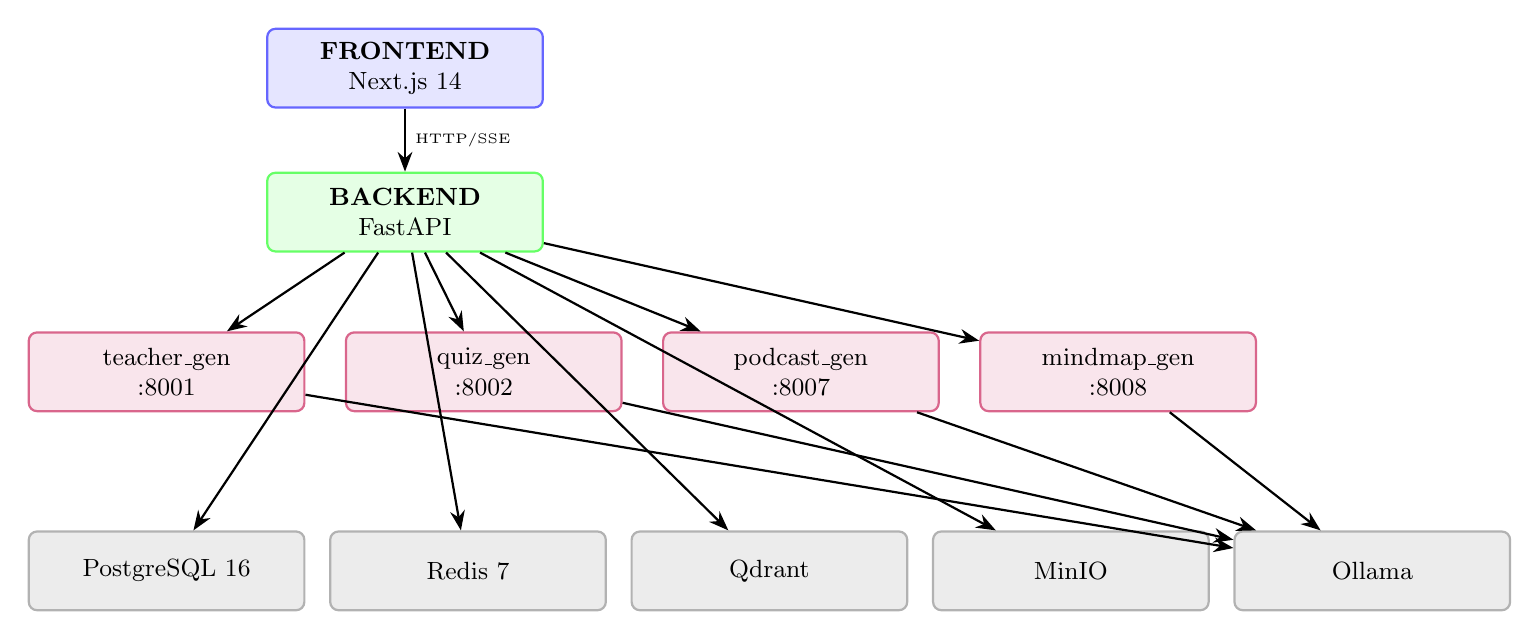
\begin{tikzpicture}[
        font=\small,
        >={Stealth[length=2.5mm]},
        node distance=8mm,
        box/.style={rectangle, rounded corners=3pt, draw, thick, minimum width=3.5cm, minimum height=1cm, align=center},
        frontend/.style={box, fill=blue!10, draw=blue!60},
        backend/.style={box, fill=green!10, draw=green!60},
        generator/.style={box, fill=purple!10, draw=purple!60},
        infra/.style={box, fill=gray!15, draw=gray!60},
        arrow/.style={->, thick}
    ]
        % Frontend layer
        \node[frontend] (frontend) {\textbf{FRONTEND}\\Next.js 14};
        
        % Backend layer
        \node[backend, below=of frontend] (backend) {\textbf{BACKEND}\\FastAPI};
        
        % Generator layer
        \node[generator, below left=10mm and -5mm of backend] (teacher) {teacher\_gen\\:8001};
        \node[generator, right=5mm of teacher] (quiz) {quiz\_gen\\:8002};
        \node[generator, right=5mm of quiz] (podcast) {podcast\_gen\\:8007};
        \node[generator, right=5mm of podcast] (mindmap) {mindmap\_gen\\:8008};
        
        % Infrastructure layer
        \node[infra, below=15mm of teacher] (postgres) {PostgreSQL 16};
        \node[infra, right=3mm of postgres] (redis) {Redis 7};
        \node[infra, right=3mm of redis] (qdrant) {Qdrant};
        \node[infra, right=3mm of qdrant] (minio) {MinIO};
        \node[infra, right=3mm of minio] (ollama) {Ollama};
        
        % Arrows
        \draw[arrow] (frontend) -- (backend) node[midway, right, font=\tiny] {HTTP/SSE};
        \draw[arrow] (backend) -- (teacher);
        \draw[arrow] (backend) -- (quiz);
        \draw[arrow] (backend) -- (podcast);
        \draw[arrow] (backend) -- (mindmap);
        
        \draw[arrow] (backend) -- (postgres);
        \draw[arrow] (backend) -- (redis);
        \draw[arrow] (backend) -- (qdrant);
        \draw[arrow] (backend) -- (minio);
        
        \draw[arrow] (teacher) -- (ollama);
        \draw[arrow] (quiz) -- (ollama);
        \draw[arrow] (podcast) -- (ollama);
        \draw[arrow] (mindmap) -- (ollama);
    \end{tikzpicture}
    \caption{Architecture globale de TeacherLM (vue simplifiée).}
\end{figure}

\subsection{Flux de données pour un message utilisateur}

\begin{enumerate}
    \item Le frontend envoie un message via \texttt{POST /api/conversations/\{id\}/chat}
    \item Le backend persiste le tour utilisateur dans \textbf{PostgreSQL}
    \item Le \textbf{Retrieval Orchestrator} sélectionne un mode de retrieval (ex: \texttt{semantic\_topk} pour le chat)
    \item \textbf{Qdrant} récupère les chunks pertinents via retrieval hybride (dense + BM25 → RRF)
    \item Le backend charge le \textbf{LearnerState} depuis PostgreSQL
    \item Le backend assemble un payload \texttt{GeneratorInput}
    \item Le \textbf{Dispatcher} route le payload vers le générateur approprié via HTTP/SSE
    \item Le générateur exécute son pipeline multi-étapes :
        \begin{itemize}
            \item Analyse de la question
            \item Reranking des chunks récupérés
            \item Génération LLM avec streaming
            \item Extraction des mises à jour du LearnerState
        \end{itemize}
    \item Le backend proxyse le stream SSE vers le frontend
    \item Le frontend affiche les tokens en temps réel
    \item Le backend persiste le tour assistant + mises à jour LearnerState
\end{enumerate}

\section{Stack technologique}

\subsection{Backend Python}

\begin{table}[H]
    \centering
    \small
    \begin{tabularx}{\textwidth}{@{}llXl@{}}
        \toprule
        \textbf{Technologie} & \textbf{Version} & \textbf{Rôle} & \textbf{Justification} \\
        \midrule
        Python & 3.14+ & Langage principal & Capacités async modernes, typing strict \\
        FastAPI & ≥0.135 & Framework REST + SSE & Meilleur framework async Python \\
        Pydantic V2 & ≥2.12 & Validation données & Schémas stricts pour tous les I/O \\
        SQLAlchemy 2.0 & ≥2.0.36 & ORM + async DB & ORM moderne avec asyncpg \\
        Alembic & ≥1.14 & Migrations DB & Évolution du schéma PostgreSQL \\
        Ollama & ≥0.4 & Inférence LLM locale & LLMs locaux, format JSON natif \\
        Qdrant & ≥1.12 & Base vectorielle & Optimisé pour similarité vectorielle \\
        fastembed & ≥0.4 & Embeddings texte & Léger, optimisé CPU \\
        rank-bm25 & ≥0.2.2 & Retrieval sparse & BM25Okapi pour recherche lexicale \\
        LlamaCloud & ≥1.0 & Parsing PDF & Conversion PDF → Markdown propre \\
        MinIO & ≥7.2 & Stockage objet & Compatible S3 pour fichiers \\
        Redis + arq & 7 / ≥0.26 & Queue tâches & Traitement background async \\
        httpx & ≥0.28 & Client HTTP & Communication avec générateurs \\
        sse-starlette & ≥2.1 & Server-Sent Events & Streaming token-by-token \\
        \bottomrule
    \end{tabularx}
    \caption{Stack backend et justifications techniques.}
\end{table}

\subsection{Frontend TypeScript}

\begin{table}[H]
    \centering
    \small
    \begin{tabularx}{\textwidth}{@{}llXl@{}}
        \toprule
        \textbf{Technologie} & \textbf{Version} & \textbf{Rôle} & \textbf{Justification} \\
        \midrule
        Next.js & 14 & Framework React & App Router, server components \\
        React & 18.3 & Bibliothèque UI & Composants avec hooks \\
        TypeScript & 5.6+ & Type safety & Détection erreurs à la compilation \\
        TailwindCSS & 3.4 & CSS utility-first & Styling rapide et cohérent \\
        Zustand & 5.0 & State management & Léger, basé hooks \\
        TanStack Query & 5.59 & Server state & Caching et sync données API \\
        Radix UI & Latest & Primitives accessibles & Composants headless \\
        react-markdown & 9.0 & Rendu Markdown & Support KaTeX et Mermaid \\
        KaTeX & 0.16 & Rendu LaTeX math & Affichage équations \\
        Mermaid & 11.4 & Rendu diagrammes & Flowcharts et diagrammes \\
        \bottomrule
    \end{tabularx}
    \caption{Stack frontend et justifications.}
\end{table}

\subsection{Modèles LLM et Embeddings}

\begin{table}[H]
    \centering
    \begin{tabularx}{\textwidth}{@{}lccX@{}}
        \toprule
        \textbf{Modèle} & \textbf{Paramètres} & \textbf{Quantisation} & \textbf{Utilisation} \\
        \midrule
        Llama 3.1 8B Instruct & 8B & Q4\_K\_M & Réponses chat, génération quiz/podcast/mindmap \\
        Llama 3.2 & 3B & Default & Analyse requêtes, extraction learner updates \\
        \addlinespace
        bge-small-en-v1.5 & --- & 384 dim & Embeddings denses pour recherche sémantique \\
        bge-reranker-base & --- & --- & Cross-encoder pour affiner pertinence chunks \\
        \bottomrule
    \end{tabularx}
    \caption{Modèles LLM et embeddings utilisés.}
\end{table}

\section{Pipeline RAG : De l'upload à la réponse}

\subsection{Pipeline d'ingestion asynchrone}

Le traitement des fichiers uploadés suit un workflow en 5 étapes géré par un worker \texttt{arq} :

\begin{figure}[H]
    \centering
    \begin{tikzpicture}[
        node distance=12mm,
        box/.style={rectangle, rounded corners, draw, thick, minimum width=2.5cm, minimum height=0.8cm, align=center},
        step/.style={box, fill=blue!10},
        final/.style={box, fill=green!15},
        error/.style={box, fill=red!15},
        arrow/.style={->, thick}
    ]
        \node[step] (upload) {Upload};
        \node[step, right=of upload] (parse) {Parse\\(LlamaCloud)};
        \node[step, right=of parse] (chunk) {Chunk};
        \node[step, right=of chunk] (embed) {Embed};
        \node[final, right=of embed] (ready) {Ready};
        \node[error, below=5mm of chunk] (failed) {Failed};
        
        \draw[arrow] (upload) -- node[above, font=\tiny] {uploaded} (parse);
        \draw[arrow] (parse) -- node[above, font=\tiny] {parsing} (chunk);
        \draw[arrow] (chunk) -- node[above, font=\tiny] {chunking} (embed);
        \draw[arrow] (embed) -- node[above, font=\tiny] {embedding} (ready);
        
        \draw[arrow, dashed] (parse) -- (failed);
        \draw[arrow, dashed] (chunk) -- (failed);
        \draw[arrow, dashed] (embed) -- (failed);
    \end{tikzpicture}
    \caption{Workflow d'ingestion asynchrone avec gestion d'erreurs.}
\end{figure}

\textbf{Détails des étapes :}
\begin{itemize}
    \item \textbf{Upload} : Fichier envoyé à MinIO, statut = \texttt{uploaded}
    \item \textbf{Parse} : LlamaCloud convertit PDF → Markdown propre, statut = \texttt{parsing}
    \item \textbf{Chunk} : Découpage en chunks avec métadonnées enrichies, statut = \texttt{chunking}
    \item \textbf{Embed} : Génération embeddings via fastembed, statut = \texttt{embedding}
    \item \textbf{Ready} : Stockage dans Qdrant, fichier prêt pour retrieval
    \item \textbf{Failed} : En cas d'erreur, statut = \texttt{failed} avec message d'erreur
\end{itemize}

Chaque transition de statut est persistée dans PostgreSQL pour permettre au frontend d'afficher la progression en temps réel.

\subsection{Retrieval hybride : 5 modes spécialisés}

Différents types de contenu nécessitent différentes stratégies de retrieval. TeacherLM implémente 5 modes optimisés :

\begin{table}[H]
    \centering
    \small
    \begin{tabularx}{\textwidth}{@{}lXlc@{}}
        \toprule
        \textbf{Mode} & \textbf{Description} & \textbf{Cas d'usage} & \textbf{k} \\
        \midrule
        semantic\_topk & Dense + BM25 + RRF & Chat, réponses directes & 12 \\
        \addlinespace
        coverage\_broad & MMR (diversité maximale) & Quiz (éviter répétitions) & 15--20 \\
        \addlinespace
        topic\_clusters & K-means sur embeddings & Résumés structurés, mind maps & Variable \\
        \addlinespace
        metadata\_filtered & Filtrage par attributs & Requêtes ciblées & 10--15 \\
        \addlinespace
        contextual\_expansion & Chunks voisins (±1) & Contexte étendu & Variable \\
        \bottomrule
    \end{tabularx}
    \caption{Modes de retrieval et leurs applications.}
\end{table}

\subsection{Reciprocal Rank Fusion (RRF)}

La force du retrieval hybride réside dans la combinaison de deux approches complémentaires via RRF :

\begin{itemize}
    \item \textbf{BM25 (sparse)} : Excellent pour les correspondances lexicales exactes (termes techniques, acronymes)
    \item \textbf{Sémantique (dense)} : Excellent pour les paraphrases et synonymes
\end{itemize}

\textbf{Formule RRF :}
\[
\text{RRF}(d) = \sum_{r \in R} \frac{1}{k + \text{rank}_r(d)}
\]
où $R = \{\text{BM25}, \text{Semantic}\}$ et $k = 60$

\textbf{Avantages :}
\begin{itemize}
    \item Sans paramètres à tuner (pas de pondération manuelle)
    \item Robuste aux variations de qualité des listes
    \item Combine forces complémentaires
    \item Performance systématiquement supérieure aux approches mono-signal
\end{itemize}

\section{Architecture multi-agents : Les générateurs}

\subsection{Vue d'ensemble des générateurs}

Chaque type de contenu pédagogique est géré par un microservice dédié. Cette architecture permet un scaling indépendant et des cycles de déploiement découplés.

\begin{table}[H]
    \centering
    \small
    \begin{tabularx}{\textwidth}{@{}llXc@{}}
        \toprule
        \textbf{Générateur} & \textbf{Port} & \textbf{Description} & \textbf{Modèles} \\
        \midrule
        teacher\_gen & 8001 & Réponses conversationnelles avec citations & 3 LLMs \\
        quiz\_gen & 8002 & QCM, vrai/faux, compléter avec distracteurs & Llama 3.1 \\
        flashcard\_gen & 8005 & Cartes mémoire recto/verso & Llama 3.1 \\
        podcast\_gen & 8007 & Script conversationnel → MP3 multi-voix & Llama 3.1 + TTS \\
        mindmap\_gen & 8008 & Carte mentale hiérarchique (JSON) & Llama 3.1 \\
        \bottomrule
    \end{tabularx}
    \caption{Générateurs spécialisés et leurs responsabilités.}
\end{table}

\subsection{Pipeline d'un générateur (exemple : teacher\_gen)}

Chaque générateur suit un pipeline multi-étapes standardisé avec streaming SSE :

\begin{enumerate}
    \item \textbf{Analysis} (Llama 3.2) : Analyse de la question et classification de l'intention
    \item \textbf{Reranking} (bge-reranker) : Affinage de la pertinence des chunks récupérés
    \item \textbf{Generation} (Llama 3.1) : Génération de la réponse avec streaming token-by-token
    \item \textbf{Learner Update} (Llama 3.2) : Extraction des mises à jour du profil d'apprenant
\end{enumerate}

\textbf{Événements SSE émis :}
\begin{itemize}
    \item \texttt{analysis} : Résultat de l'analyse de la question
    \item \texttt{sources} : Chunks récupérés et reranked
    \item \texttt{token} : Tokens de la réponse (streaming)
    \item \texttt{done} : Métadonnées finales + learner updates
\end{itemize}

\subsection{Règle d'ancrage stricte}

Tous les générateurs incluent la règle de grounding suivante dans leur prompt système :

\begin{quote}
\textit{``Base your response EXCLUSIVELY on the COURSE MATERIAL. Never fabricate information. If the material doesn't cover the topic, say so explicitly.''}
\end{quote}

Cette règle garantit que le système ne peut pas halluciner à partir de ses connaissances pré-entraînées.

\section{Suivi de l'apprenant (Learner Tracking)}

\subsection{Structure LearnerState}

Chaque conversation maintient un état d'apprentissage persistant :

\begin{lstlisting}[language=Python]
class LearnerState:
    understood_concepts: list[str]
    struggling_concepts: list[str]
    mastery_scores: dict[str, float]  # {concept: score}
    question_history: list[str]
    last_updated: datetime
\end{lstlisting}

\subsection{Calcul du score de maîtrise}

Le score de maîtrise d'un concept $c$ est calculé comme une moyenne pondérée temporellement :

\[
M(c) = \frac{1}{N}\sum_{i=1}^{N} w_i \cdot s_i
\]

où :
\begin{itemize}
    \item $s_i$ : score de l'interaction $i$
    \item $w_i$ : poids temporel (les interactions récentes pèsent plus lourd)
    \item $N$ : nombre d'interactions sur le concept
\end{itemize}

\subsection{Extraction automatique des mises à jour}

Après chaque réponse, Llama 3.2 analyse la conversation pour extraire :
\begin{itemize}
    \item Concepts mentionnés dans la question
    \item Signes de compréhension ou confusion
    \item Nouveaux concepts introduits
\end{itemize}

Le JSON structuré est généré via le paramètre \texttt{format=} d'Ollama (pas besoin de parsing manuel).

\subsection{Adaptation pédagogique}

Le LearnerState influence directement la génération de contenu :

\begin{table}[H]
    \centering
    \small
    \begin{tabularx}{\textwidth}{@{}lX@{}}
        \toprule
        \textbf{Générateur} & \textbf{Adaptation basée sur LearnerState} \\
        \midrule
        Quiz & Difficulté progressive basée sur \texttt{mastery\_scores}. Focus sur \texttt{struggling\_concepts}. Évite concepts dans \texttt{understood\_concepts} (score $> 0.8$). \\
        \addlinespace
        Chat & Ton encourageant si \texttt{struggling\_concepts} nombreux. Références aux concepts déjà compris. Indices socratiques pour concepts difficiles. \\
        \addlinespace
        Podcast & Script adapté au niveau de maîtrise général. Tempo et profondeur ajustés dynamiquement. \\
        \bottomrule
    \end{tabularx}
    \caption{Stratégies d'adaptation par générateur.}
\end{table}

\section{Exemples de générateurs spécialisés}

\subsection{Quiz Generator}

\textbf{Types de questions :}
\begin{itemize}
    \item \textbf{MCQ} : 4 choix, 1 correcte + 3 distracteurs plausibles
    \item \textbf{Vrai/Faux} : Affirmation + explication
\end{itemize}

\textbf{Stratégie de génération :}
\begin{enumerate}
    \item Retrieval mode \texttt{coverage\_broad} (MMR) pour diversité
    \item Filtrage par \texttt{struggling\_concepts} si disponible
    \item Génération JSON structuré (schéma Pydantic)
    \item Validation : pas de doublons, distracteurs différents
    \item Sauvegarde MinIO + métadonnées PostgreSQL
\end{enumerate}

\subsection{Podcast Generator}

\textbf{Pipeline de génération :}
\begin{enumerate}
    \item \textbf{Retrieval} : Mode \texttt{topic\_clusters} pour couverture thématique
    \item \textbf{Script} : Llama 3.1 génère dialogue conversationnel (2 voix : hôte + invité)
    \item \textbf{TTS} : Synthèse vocale avec voix distinctes (masculin/féminin)
    \item \textbf{Mixing} : Fusion audio avec pauses naturelles
    \item \textbf{Export} : MP3 sauvé dans MinIO
\end{enumerate}

\textbf{Paramètres configurables :}
\begin{itemize}
    \item Durée cible : 5--30 minutes
    \item Niveau technique : débutant/intermédiaire/avancé
    \item Langue : multilingue via TTS
\end{itemize}

\subsection{Mind Map Generator}

\textbf{Structure JSON hiérarchique :}
\begin{lstlisting}[language=json]
{
  "root": {"label": "Neural Networks", "id": "root"},
  "branches": [
    {
      "label": "Architecture",
      "children": [
        {"label": "Layers"},
        {"label": "Activations"}
      ]
    },
    {
      "label": "Training",
      "children": [
        {"label": "Backprop"},
        {"label": "Optimizers"}
      ]
    }
  ]
}
\end{lstlisting}

\textbf{Rendu frontend :}
\begin{itemize}
    \item Visualisation interactive (D3.js / Mermaid)
    \item Zoom / pan
    \item Export SVG / PNG
\end{itemize}

\section{Infrastructure et déploiement}

\subsection{Architecture Docker Compose}

Tous les services sont conteneurisés et orchestrés via Docker Compose :

\begin{table}[H]
    \centering
    \begin{tabularx}{\textwidth}{@{}lccX@{}}
        \toprule
        \textbf{Service} & \textbf{Port} & \textbf{Technologie} & \textbf{Rôle} \\
        \midrule
        Frontend & 3000 & Next.js 14 & Interface utilisateur \\
        Backend & 8000 & FastAPI & API REST + SSE \\
        teacher\_gen & 8001 & FastAPI & Générateur chat \\
        quiz\_gen & 8002 & FastAPI & Générateur quiz \\
        podcast\_gen & 8007 & FastAPI & Générateur podcast \\
        mindmap\_gen & 8008 & FastAPI & Générateur mind map \\
        \midrule
        PostgreSQL & 5432 & PostgreSQL 16 & Base relationnelle \\
        Redis & 6379 & Redis 7 & Queue tâches + cache \\
        Qdrant & 6333/6334 & Qdrant & Base vectorielle \\
        MinIO & 9000/9001 & MinIO & Stockage objet (S3) \\
        \bottomrule
    \end{tabularx}
    \caption{Services Docker et leurs ports.}
\end{table}

\subsection{Volumes persistants}

\begin{itemize}
    \item \texttt{postgres\_data} : Données PostgreSQL
    \item \texttt{qdrant\_data} : Embeddings vectoriels
    \item \texttt{minio\_data} : Fichiers uploadés et artefacts générés
    \item \texttt{fastembed\_cache} : Modèles d'embedding téléchargés
    \item \texttt{hf\_cache} : Cache HuggingFace
\end{itemize}

\subsection{Commandes de déploiement}

\begin{lstlisting}[language=bash]
# Demarrage complet (build si necessaire)
./run.sh up

# Rebuild complet depuis zero
./run.sh rebuild

# Consultation logs
./run.sh logs [service_name]

# Arret de tous les services
./run.sh stop
\end{lstlisting}

\subsection{Prérequis : Ollama sur l'hôte}

Ollama doit être installé et fonctionnel sur la machine hôte avec les modèles suivants :

\begin{lstlisting}[language=bash]
ollama pull llama3.1:8b-instruct-q4_K_M
ollama pull llama3.2:latest
\end{lstlisting}

Les services Docker accèdent à Ollama via \texttt{host.docker.internal:11434}.

\section{Décisions architecturales clés}

\subsection{Pourquoi des LLM locaux (Ollama) plutôt qu'OpenAI ?}

\begin{table}[H]
    \centering
    \begin{tabularx}{\textwidth}{@{}lX@{}}
        \toprule
        \textbf{Raison} & \textbf{Bénéfice} \\
        \midrule
        Confidentialité & Les documents de cours ne quittent jamais la machine \\
        Coût & Pas de frais par token -- utilisation illimitée après provisionnement \\
        Transparence & Reproductible, pas de vendor lock-in \\
        Offline & Fonctionne sans internet (après téléchargement modèles) \\
        \bottomrule
    \end{tabularx}
\end{table}

\subsection{Pourquoi pas LangChain / LangGraph ?}

\begin{itemize}
    \item \textbf{Avertissements Pydantic V1} : Incompatibilité avec Python 3.14 en mode strict
    \item \textbf{Abstraction inutile} : Le paramètre \texttt{format=} d'Ollama pour JSON structuré remplace toute la complexité des chains
    \item \textbf{Simplicité de débogage} : Contrôle total sur chaque appel LLM sans boîte noire
\end{itemize}

\subsection{Pourquoi une architecture microservices par générateur ?}

\begin{table}[H]
    \centering
    \begin{tabularx}{\textwidth}{@{}lX@{}}
        \toprule
        \textbf{Avantage} & \textbf{Explication} \\
        \midrule
        Scaling indépendant & teacher\_gen (temps réel) vs quiz\_gen (batch) ont des besoins différents \\
        Déploiement indépendant & Mise à jour du pipeline quiz sans redémarrer le chat \\
        Modèles différents & Chaque générateur utilise ses propres configurations Ollama \\
        Extensibilité & Ajout de nouveaux générateurs sans modifier le code existant \\
        \bottomrule
    \end{tabularx}
\end{table}

\subsection{Pourquoi Reciprocal Rank Fusion (RRF) ?}

\begin{itemize}
    \item Les embeddings denses excellent en \textbf{similarité sémantique} mais ratent les \textbf{correspondances exactes}
    \item BM25 excelle en \textbf{matching lexical} mais rate les \textbf{paraphrases}
    \item RRF est une méthode de fusion sans paramètres qui produit systématiquement de meilleurs résultats
\end{itemize}

\subsection{Pourquoi 5 modes de retrieval ?}

Différents types de sorties ont des besoins informationnels fondamentalement différents :

\begin{itemize}
    \item Chat : chunks les \textbf{plus pertinents} (semantic\_topk)
    \item Quiz : \textbf{couverture large} pour éviter questions répétitives (coverage\_broad / MMR)
    \item Rapports : \textbf{structure thématique} (topic\_clusters / K-means)
\end{itemize}

\section{Base de données PostgreSQL}

\subsection{Schéma relationnel}

\begin{table}[H]
    \centering
    \small
    \begin{tabularx}{\textwidth}{@{}lX@{}}
        \toprule
        \textbf{Table} & \textbf{Description} \\
        \midrule
        users & Authentification, profils utilisateurs \\
        conversations & Sessions de chat (1 par contexte d'apprentissage) \\
        messages & Messages utilisateur/assistant dans conversations \\
        files & Fichiers uploadés + statut ingestion (uploaded → ready) \\
        learner\_states & État d'apprentissage par conversation (1:1) \\
        artifacts & Quiz, podcasts, mind maps générés \\
        concept\_mastery & Scores de maîtrise par concept et utilisateur \\
        \bottomrule
    \end{tabularx}
    \caption{Tables principales de PostgreSQL.}
\end{table}

\subsection{Relations clés}

\begin{itemize}
    \item \texttt{conversations} $\rightarrow$ \texttt{users} (N:1)
    \item \texttt{messages} $\rightarrow$ \texttt{conversations} (N:1)
    \item \texttt{files} $\rightarrow$ \texttt{conversations} (N:1)
    \item \texttt{learner\_states} $\leftrightarrow$ \texttt{conversations} (1:1)
    \item \texttt{artifacts} $\rightarrow$ \texttt{conversations} (N:1)
\end{itemize}

\subsection{Migrations avec Alembic}

Le schéma évolue via migrations versionnées :

\begin{lstlisting}[language=bash]
# Generer une migration
alembic revision --autogenerate -m "Add concept_mastery table"

# Appliquer les migrations
alembic upgrade head

# Rollback
alembic downgrade -1
\end{lstlisting}

\section{Évolution du projet}

\subsection{Phase 1 : Prototype RAG classique}

\begin{itemize}
    \item RAG monolithique avec Mistral-7B et ChromaDB
    \item Retrieval sémantique seul
    \item Chat uniquement
    \item Interface CLI
\end{itemize}

\subsection{Phase 2 : Système agentique}

\begin{itemize}
    \item Transition vers LangGraph
    \item Retrieval hybride (BM25 + sémantique)
    \item 5 outils spécialisés
    \item Support multilingue
\end{itemize}

\subsection{Phase 3 : Architecture microservices}

\begin{itemize}
    \item Séparation en générateurs indépendants
    \item Passage à Llama 3.1/3.2 via Ollama
    \item Infrastructure Docker complète
\end{itemize}

\subsection{Phase 4 : Plateforme de production (actuel)}

\begin{itemize}
    \item Interface web Next.js professionnelle
    \item 5 générateurs de contenu
    \item Suivi pédagogique (LearnerState)
    \item Base PostgreSQL + Redis + Qdrant + MinIO
    \item Déploiement Docker Compose
\end{itemize}

\section{Défis techniques rencontrés}

\subsection{Hallucinations résiduelles}

\textbf{Problème :} Même avec grounding strict, le LLM peut occasionnellement générer du contenu non supporté par les chunks.

\textbf{Solution :} Post-traitement déterministe qui vérifie la cohérence entre chunks récupérés et réponse générée. En cas de détection d'hallucination, repli sur réponse déterministe.

\subsection{Parsing PDF complexe}

\textbf{Problème :} PDFs avec multi-colonnes, équations, tableaux difficiles à extraire proprement.

\textbf{Solution :} Migration vers LlamaCloud qui produit Markdown structuré de haute qualité. Alternative locale : PyMuPDF avec post-processing.

\section{Conclusion}

TeacherLM démontre qu'un système de tutorat IA avancé, entièrement local et respectueux de la vie privée, est techniquement viable et pédagogiquement efficace.

\subsection{Contributions principales}

\begin{enumerate}
    \item \textbf{Pipeline RAG éducatif complet} : De l'upload à la génération multi-modale
    \item \textbf{Retrieval hybride performant} : BM25 + dense + RRF avec 5 modes spécialisés
    \item \textbf{LearnerState tracking automatisé} : Adaptation pédagogique basée données
    \item \textbf{Architecture plugin microservices} : Extensible et scalable
    \item \textbf{Intégration Ollama production} : LLMs locaux haute performance
    \item \textbf{Streaming SSE token-by-token} : Expérience utilisateur fluide
    \item \textbf{Multi-modal outputs} : Texte, audio (podcasts), visualisations (mind maps), évaluations (quiz)
\end{enumerate}

\subsection{Impact}

TeacherLM prouve que l'IA éducative peut être :
\begin{itemize}
    \item \textbf{Fiable} : Zéro hallucination grâce au grounding strict
    \item \textbf{Privée} : Données qui ne quittent jamais la machine
    \item \textbf{Adaptative} : Suivi pédagogique intelligent
    \item \textbf{Accessible} : Pas de coûts récurrents API
    \item \textbf{Transparente} : Code et modèles open source
\end{itemize}

\subsection{Mot de la fin}

Ce projet a transformé un prototype RAG basique en une plateforme de production complète. L'architecture microservices, le retrieval hybride, et le suivi pédagogique adaptatif positionnent TeacherLM comme une solution viable pour l'éducation assistée par IA, tout en garantissant confidentialité et contrôle total des données.

\end{document}